\documentclass{beamer}
\usetheme{Singapore}
\setbeamertemplate{navigation symbols}{}

% Packages
  % General packages
  \usepackage[utf8x]{inputenc} % Danish language support
  \usepackage[light]{antpolt} % Provides awesome font
  \usepackage{hyperref} % Provides \url and clickable links in the pdf
  \usepackage{cleveref}	% Provides \cref and \Cref for including text before references
  \usepackage{graphicx}	% Provides the \includegraphics[]{} command
  \usepackage{comment} % Provides comment-environment for multi-line commenting
  \usepackage{twoopt} % Allows adding commands with two optional arguments
  \usepackage{setspace} % Provides onehalfspacing environment
  \usepackage{enumitem}	% Provides control of spacing in lists
  \usepackage{amsbsy} % Provides \boldsymbol command
  \usepackage{lipsum} % Provides \lipsum command
  \usepackage{apacite} % Provides bibliography style
	
  % Math packages
  \usepackage{amsmath, amssymb, amsfonts} % Math symbolic jargon
  \usepackage{amsthm} % Theorem environment
  \usepackage{mathrsfs}	% Provides the \mathscr{} curly font
  \usepackage{stmaryrd}	% Provides the \lightning symbol and semantics-brackets, among others
  \usepackage{tikz} % Awesome diagrams
  \usepackage{tikz-cd} % For making tree cds
    \usetikzlibrary{matrix,arrows} % Matrices and arrows for style points
    \usetikzlibrary{decorations.pathreplacing,calc,arrows.meta} % For making tree cds
  %\usepackage[all]{xy} % Provides xymatrix environment for diagrams

  % Beamer packages
  \usepackage[absolute,overlay]{textpos}  % Placement of textblocks
  \usepackage{mathdots}  % Provides \iddots command

% Tree diagrams
\tikzset{
  tree/.style 2 args={
    decorate,
    decoration={
      show path construction,
      lineto code={
        \draw[dotted,-] (\tikzinputsegmentfirst) --($(\tikzinputsegmentfirst)!.5!(\tikzinputsegmentlast)$);
        \draw[-{Latex}] ($(\tikzinputsegmentfirst)!.5!(\tikzinputsegmentlast)$) --(\tikzinputsegmentlast) node [midway,right] {\small{$#1$}};
        \draw[-] (\tikzinputsegmentfirst) --++ (105:0.65cm);
        \draw[-] (\tikzinputsegmentfirst) --++ (75:0.65cm) node [midway, right] {\small{$#2$}};
      }
    }
  }
}

% User-defined commands
  % General things	
  \newcommand{\eq}[1]{\begin{align*} #1 \end{align*}}
  \newcommand{\eqq}[1]{\begin{align*} #1\\ \end{align*}}
  \newcommand{\pic}[1]{\begin{center}\includegraphics[scale=.5]{#1}\\\end{center}}
  \newcommand{\pix}[2]{\begin{center}\includegraphics[scale=#2]{#1}\\\end{center}}
  %\newcommand{\cd}[1]{\eq{\xymatrix@L=6pt{#1}}}
  \renewcommand{\b}[1]{{\bf #1}}

  % Declared operators
  \DeclareMathOperator{\rud}{rud}
  \DeclareMathOperator{\pred}{pred}
  \DeclareMathOperator{\card}{card}
  \DeclareMathOperator{\on}{On}
  \DeclareMathOperator{\val}{val}
  \DeclareMathOperator{\ran}{ran}
  \DeclareMathOperator{\cod}{cod}
  \DeclareMathOperator{\trcl}{trcl}
  \DeclareMathOperator{\dom}{dom}	
  \DeclareMathOperator{\rank}{rank}
  \DeclareMathOperator{\im}{im}
  \DeclareMathOperator{\ma}{MA}
  \DeclareMathOperator{\hull}{Hull}
  \DeclareMathOperator{\chull}{cHull}
  \DeclareMathOperator{\id}{id}
  \DeclareMathOperator{\cof}{cof}
  \DeclareMathOperator{\Th}{Th}
  \DeclareMathOperator{\sing}{Sing}
  \DeclareMathOperator{\cl}{cl}
  \DeclareMathOperator{\Int}{int}
  \DeclareMathOperator{\ob}{Ob}
  \DeclareMathOperator{\col}{Col}
  \DeclareMathOperator{\sat}{Sat}
  \DeclareMathOperator{\lh}{lh}
  \DeclareMathOperator{\mor}{Mor}
  \DeclareMathOperator{\ult}{Ult}
  \DeclareMathOperator{\comp}{\textsf{Comp}}
  \DeclareMathOperator{\zf}{\mathsf{ZF}}
  \DeclareMathOperator{\zfc}{\mathsf{ZFC}}
  \DeclareMathOperator{\ch}{\mathsf{CH}}
  \DeclareMathOperator{\gch}{\mathsf{GCH}}
  \DeclareMathOperator{\con}{Con}
  \DeclareMathOperator{\cf}{cf}
  \DeclareMathOperator{\crit}{crit}
  \DeclareMathOperator{\pd}{pd}
  \DeclareMathOperator{\ad}{\mathsf{AD}}
  \DeclareMathOperator{\ac}{\mathsf{AC}}
  \DeclareMathOperator{\xor}{\oplus}
  \DeclareMathOperator{\nor}{\downarrow}
  \DeclareMathOperator{\nand}{\uparrow}
  \DeclareMathOperator{\biglor}{\bigvee}
  \DeclareMathOperator{\bigland}{\bigwedge}
  \DeclareMathOperator{\Lr}{\Leftrightarrow}
  \DeclareMathOperator{\lr}{\leftrightarrow}
  \DeclareMathOperator{\ip}{\perp\!\!\!\perp}
  \DeclareMathOperator{\psubset}{\subsetneq}
  \DeclareMathOperator{\psupset}{\supsetneq}
  \DeclareMathOperator{\elsub}{\prec}
  \DeclareMathOperator{\elsup}{\succ}
  \DeclareMathOperator{\contr}{\lightning}
  \DeclareMathOperator{\proves}{\vdash}
  \DeclareMathOperator{\nproves}{\nvdash}
  \DeclareMathOperator{\nmodels}{\nvDash}
  \DeclareMathOperator{\forces}{\Vdash}
  \DeclareMathOperator{\nforces}{\nVdash}
  \DeclareMathOperator{\adj}{\dashv}
  \DeclareMathOperator{\restr}{\upharpoonright}
  \DeclareMathOperator{\ex}{\underline{ex}}
  \DeclareMathOperator{\st}{\underline{st}}
  \DeclareMathOperator{\sv}{\underline{sv}}
  \DeclareMathOperator{\tl}{\underline{tl}}
  \DeclareMathOperator{\tensor}{\otimes}
  \DeclareMathOperator{\M}{\mathcal{M}}
  \DeclareMathOperator{\N}{\mathcal{N}}
  \DeclareMathOperator{\Q}{\mathcal{Q}}
  \DeclareMathOperator{\R}{\mathcal{R}}
  \DeclareMathOperator{\W}{\mathcal{W}}
  \DeclareMathOperator{\F}{\mathcal{F}}
  \DeclareMathOperator{\T}{\mathcal{T}}
  \DeclareMathOperator{\U}{\mathcal{U}}
  \DeclareMathOperator{\V}{\mathcal{V}}
  \DeclareMathOperator{\G}{\mathcal{G}}
  \DeclareMathOperator{\A}{\mathcal{A}}
  \DeclareMathOperator{\pr}{pr}
  \DeclareMathOperator{\Root}{root}
  \DeclareMathOperator{\wfp}{wfp}
  \DeclareMathOperator{\Def}{Def}

  % Redeclared operators
  \renewcommand{\subset}{\subseteq}
  \renewcommand{\supset}{\supseteq}
  \newcommand{\nsubset}{\nsubseteq}
  \newcommand{\nsupset}{\nsupseteq}
  \renewcommand{\hom}{\text{Hom}}
  \renewcommand{\P}{\mathcal{P}}
  \renewcommand{\S}{\mathcal{S}}
  \renewcommand{\H}{\mathcal{H}}
  \renewcommand{\succ}{\text{succ}}

  % Convenient shortcuts
  \newcommand{\vto}[2]{\begin{pmatrix}#1\\#2\end{pmatrix}}
  \newcommand{\vtre}[3]{\begin{pmatrix}#1\\#2\\#3\end{pmatrix}}
  \newcommand{\mto}[4]{\begin{pmatrix} #1 & #2 \\ #3 & #4\end{pmatrix}}
  \newcommand{\mtre}[9]{\begin{pmatrix} #1 & #2 & #3 \\ #4 & #5 & #6 \\ #7 & #8 & #9\end{pmatrix}}
  \newcommand{\bra}[1]{\langle #1\rangle}
  \newcommand{\dbra}[1]{\llbracket #1 \rrbracket}
  \newcommand{\norm}[1]{\left|\left|#1\right|\right|}
  \newcommand{\abs}[1]{\left|#1\right|}
  \newcommand{\normal}{\unlhd}
  \newcommand{\ideal}{\unlhd}
  \newcommand{\init}{\unlhd}
  \newcommand{\core}{\mathfrak C}
  \newcommand{\E}{\vec{E}}
  \newcommand{\J}{\mathcal{J}}
  \newcommand{\rel}{\ \text{rel}\ }
  \newcommand{\pnormal}{\mathrel{\ooalign{$\lneq$\cr\raise.22ex\hbox{$\lhd$}\cr}}}
  \newcommand{\pideal}{\mathrel{\ooalign{$\lneq$\cr\raise.22ex\hbox{$\lhd$}\cr}}}
  \newcommand{\pinit}{\lhd}
  \newcommand{\acts}{\curvearrowright}
  \newcommand{\colimm}{\varinjlim}
  \newcommand{\limm}{\varprojlim}
  \newcommand{\set}{\textsf{Set}}
  \newcommand{\godel}[1]{\ulcorner #1 \urcorner}
  \newcommand{\game}[8]{\eq{\begin{array}{ccccccccc} \text{I} & #1 && #3 && #5 && #7\\ \text{II} && #2 && #4 && #6 && #8 \end{array}}}
  \newcommand{\bgame}[8]{\eq{\begin{array}{ccccccccc} \text{I} & #1 & #3 & #5 & #7 \\ \text{II} & #2 & #4 & #6 & #8 \end{array}}}
  \newcommand{\los}{{{\fontfamily{arial}\selectfont\L}o\' s}}


\title{{\scshape\small Pure Postgraduate Seminar}\\ Inner Model Theory}
\author{Dan Saattrup Nielsen}
\date{\small December 9, 2016}

\begin{document}

{\setbeamertemplate{background canvas}{\tikz[remember picture,overlay,shift={(current page.center)}]\node[opacity=0.7] at (4.5,-4) {
\includegraphics[scale=0.15]{UoBlogo.png}};}

\begin{frame}
  \maketitle
\end{frame}}

\begin{frame}{What's inner model theory?}
\begin{center}
\begin{tikzpicture}

  \onslide<2-5>
  \node at (0.5,0) {$\emptyset$};
  
  \onslide<2-7>
  \node at (0,0) {$\bullet$};

  \onslide<3-7>
  \node at (0,1) {$\bullet$};

  \onslide<3-5>
  \node at (0.6,1) {$\{\emptyset\}$};

  \onslide<4-7>
  \node at (-0.5,2) {$\bullet$};
  \node at (0.5,2) {$\bullet$};

  \onslide<4-5>
  \node at (-1.5,2) {$\{\emptyset,\{\emptyset\}\}$};
  \node at (1.4,2) {$\{\{\emptyset\}\}$};

  \onslide<5-7>
  \node at (-0.9,3) {$\bullet$};
  \node at (-0.3,3) {$\bullet$};
  \node at (0.9,3) {$\bullet$};
  \node at (0.3,3) {$\bullet$};

  \onslide<6-7>
  \node at (0,4) {$\vdots$};
  
  \onslide<7->
  \draw (-2.3,6) -- (0,0) -- (2.3,6);

  \onslide<8->
  \node at (1.7,3) {$V$};
 
  \onslide<9-10>
  \node at (0,0.7) {$1$};
  \node at (0,1.2) {$2$};
  \node at (0,1.7) {$3$};
  \node at (0,2.3) {$\vdots$};
  \node at (0,2.7) {$\mathbb N$};
  \node at (0.8,3.5) {$\mathbb C$};
  \node at (0.2,3.3) {$\mathbb R$};
  \node at (-0.5,3.9) {$\mathbb R^{\mathbb R^{\mathbb R^{\iddots}}}$};
  \node at (0,5) {$\vdots$};

  \onslide<10-12>
  \node at (1.5,5.6) {?};

  \onslide<12>
  \draw[blue] (-1.2,6) -- (0,0) -- (1.2,6);
  \node at (-0.4,3.5) {$\color{blue}L$};

  \onslide<13>
  \draw[blue] (-1.5,6) -- (0,0) -- (1.5,6);
  \node at (1.7,5.6) {?};

  \onslide<14>
  \draw[blue] (-1.8,6) -- (0,0) -- (1.8,6);
  \node at (1.9,5.6) {?};

\end{tikzpicture}
\end{center}
\end{frame}

\begin{frame}{What's inner model theory?}
\begin{center}
\begin{tikzpicture}
  
  \onslide<1->
  \node at (0,0) {$\bullet$};
  \node at (0,0.5) {$\bullet$};
  \node at (0,1) {$\bullet$};
  \node at (0,1.5) {$\bullet$};
  \node at (0,2) {$\bullet$};
  \node at (0,2.5) {$\bullet$};
  \node at (0,3) {$\bullet$};
  \node at (0,3.5) {$\bullet$};
  \node at (1,4.3) {$\bullet$};
  \node at (-1,4.3) {$\bullet$};
  \node at (0,5) {$\bullet$};
  \node at (0,5.5) {$\bullet$};
  \node at (0,6) {$\bullet$};
  \node at (0,6.5) {$\vdots$};
  \node at (2.5,0) {\parbox{4cm}{\footnotesize Inaccessible}};
  \node at (2.5,0.5) {\parbox{4cm}{\footnotesize Mahlo}};
  \node at (2.5,1) {\parbox{4cm}{\footnotesize Weakly compact}};
  \node at (2.5,1.5) {\parbox{4cm}{\footnotesize Indescribable}};
  \node at (2.5,2) {\parbox{4cm}{\footnotesize Ramsey}};
  \node at (2.5,2.5) {\parbox{4cm}{\footnotesize Measurable}};
  \node at (2.5,3) {\parbox{4cm}{\footnotesize Strong}};
  \node at (3.4,4.3) {\parbox{4cm}{\footnotesize Superstrong}};
  \node at (-2.5,4.3) {\footnotesize Strongly compact};
  \node at (2.5,5.5) {\parbox{4cm}{\footnotesize Extendible}};
  \node at (2.5,6) {\parbox{4cm}{\footnotesize Huge}};
  \draw (0,0) -- (0,0.5) -- (0,1) -- (0,1.5) -- (0,2) -- (0,2.5) -- (0,3) -- (0,3.5);
  \draw (0,3.5) -- (1,4.3) -- (0,5) -- (-1,4.3) -- (0,3.5);
  \draw (0,5) -- (0,5.5) -- (0,6);

  \onslide<1-3>
  \node at (2.5,3.5) {\parbox{4cm}{\footnotesize Woodin}};
  
  \onslide<1-4>
  \node at (2.5,5) {\parbox{4cm}{\footnotesize Supercompact}};
  
  \onslide<2->
  \draw[thick,blue,->] (-3,0) -- (-3,3);
  \node at (-4,1.5) {\color{blue}\small Strength};

  \onslide<3>
  \node at (0,4.3) {?};

  \onslide<4>
  \node at (2.5,3.5) {\parbox{4cm}{\color{olive}\footnotesize Woodin}};
  
  \onslide<5>
  \node at (2.5,3.5) {\parbox{4cm}{\footnotesize Woodin}};
  \node at (2.5,5) {\parbox{4cm}{\footnotesize\color{red} Supercompact}};
  
  \onslide<6>
  \node at (2.5,3.5) {\parbox{4cm}{\color{olive}\footnotesize Woodin}};
  \node at (2.5,5) {\parbox{4cm}{\footnotesize Supercompact}};
  
\end{tikzpicture}
\end{center}
\end{frame}

\begin{frame}{Elementary embeddings}
\begin{center}
\begin{tikzpicture}

  \onslide<2->
  \node at (0,-0.5) {$\M$};
  \draw (0,0) -- (0,4);
  
  \onslide<2-7>
  \node at (5.5,-0.5) {$\N$};

  \onslide<2-7>
  \draw (5.5,0) -- (5.5,4);

  \onslide<11->
  \draw (5.5,0) -- (5.5,5);

  \onslide<3-7>
  \node at (2.7,-0.2) {$j$};
  \draw[->] (0.5,-0.5) -- (5,-0.5);

  \onslide<4-5>
  \node at (-0.6,-0.5) {$f\in$};
  \node at (-0.5,1) {$\beta$};
  \node at (-0.5,2) {$\alpha$};
  \draw (-0.1,1) -- (0.1,1);
  \draw (-0.1,2) -- (0.1,2);
  \node at (-0.7,-1.7) {$\M\models``f:\alpha\to\beta"$};
  
  \onslide<5>
  \node at (6.2,1.5) {$j(\beta)$};
  \node at (6.2,3) {$j(\alpha)$};
  \draw (5.4,1.5) -- (5.6,1.5);
  \draw (5.4,3) -- (5.6,3);
  \draw[->] (0.5,1) -- (5,1.5);
  \draw[->] (0.5,2) -- (5,3);
  \node at (5.5,-1.7) {$\N\models``j(f):j(\alpha)\to j(\beta)"$};

  \onslide<6-7>
  \node at (-0.7,-1.7) {\footnotesize $\M\models$``The dress is white and gold"};

  \onslide<7>
  \node at (5,-1.9) {\footnotesize $\N\models$``The dress is $\underbrace{j(\text{white})}_{\text{blue}}$ and $\underbrace{j(\text{gold})}_{\text{black}}$"};

  \onslide<9>
  \node at (-0.7,-0.5) {$E\in$};

  \onslide<10->
  \draw (0.1,1) -- (-0.1,1) -- (-0.1,2.5) -- (0.1,2.5);
  \node at (-0.5,1.8) {$E$};
  
  \onslide<11-> 
  \node at (5.5,-0.5) {$\ult(\M,E)$};
  \draw[->] (0.3,1) -- (5.2,3.5);
  \draw (5.4,3.5) -- (5.6,3.5);

\end{tikzpicture}
\end{center}
\end{frame}

\begin{frame}{Premice}
\begin{block}{Definition}
A (coarse) \textbf{premouse} is a structure of the form $\M=\bra{L_\alpha^{\E},\E,F}$, where $\E$ is a \textit{fine} extender sequence and every proper initial segment of $\M$ is {\color{orange}sound}.\\
\end{block}

\begin{center}
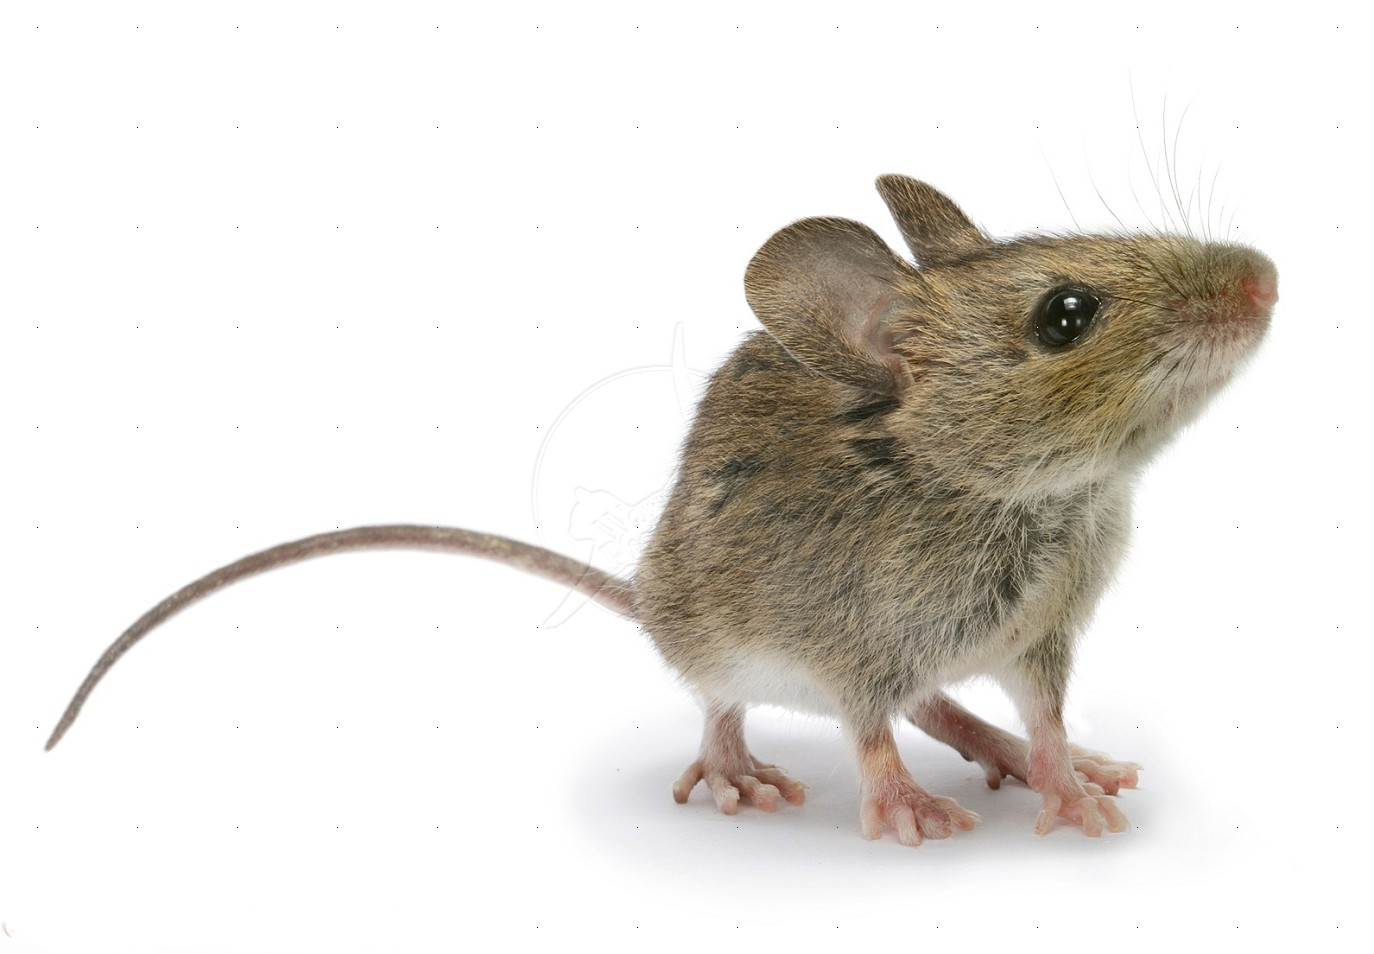
\includegraphics[scale=0.08]{gfx/mouse.jpg}\hspace{0.5cm}
\begin{tikzpicture}
  
  \node at (-1.4,1) {$=$};
  \node at (0,0) {$\M$};
  \draw (0,0.5) -- (0,3);
  \draw (-0.1,1) -- (0.2,1) -- (0.2,1.6) -- (-0.1,1.6);
  \draw (0.1,1.4) -- (-0.2,1.4) -- (-0.2,2.3) -- (0.1,2.3);
  \draw (-0.1,2) -- (0.2,2) -- (0.2,3) -- (-0.1,3);

\end{tikzpicture}
\end{center}
\end{frame}

\begin{frame}{Linear iterations}
\begin{center}
\begin{tikzpicture}
  
  \onslide<2->
  \node at (0,0) {$\M$};
  \draw (0,0.5) -- (0,3);
  \draw (-0.1,1) -- (0.1,1) -- (0.1,1.5) -- (-0.1,1.5);
  \draw (-0.1,1.8) -- (0.1,1.8) -- (0.1,2.1) -- (-0.1,2.1);

  \onslide<3>
  \node at (2,0) {$\color{red}\M_1$};
  \draw[red] (-0.1,1) -- (0.1,1) -- (0.1,1.5) -- (-0.1,1.5);
  \draw[->,red] (0.2,1) -- (1.8,1.8);
  \draw[red] (2,0.5) -- (2,3.4);
  
  \onslide<4->
  \node at (2,0) {$\M_1$};
  \draw (2,0.5) -- (2,3.4);
  \draw[->] (0.2,1) -- (1.8,1.8);
  \draw (1.9,1.8) -- (2.1,1.8) -- (2.1,2.2) -- (1.9,2.2);

  \onslide<4>
  \draw (1.9,2.6) -- (2.1,2.6) -- (2.1,3) -- (1.9,3);
  
  \onslide<5>
  \node at (4,0) {$\color{red}\M_2$};
  \draw[red] (4,0.5) -- (4,3.8);
  \draw[->,red] (2.2,2.6) -- (3.8,3.1);
  \draw[red] (1.9,2.6) -- (2.1,2.6) -- (2.1,3) -- (1.9,3);

  \onslide<6->
  \draw (1.9,2.6) -- (2.1,2.6) -- (2.1,3) -- (1.9,3);
  \node at (4,0) {$\M_2$};
  \draw (4,0.5) -- (4,3.8);
  \draw[->] (2.2,2.6) -- (3.8,3.1);
  \draw (3.9,3.1) -- (4.1,3.1) -- (4.1,3.5) -- (3.9,3.5);
  \draw (3.9,1.8) -- (4.1,1.8) -- (4.1,2.2) -- (3.9,2.2);

  \onslide<7->
  \node at (5.5,0) {$\cdots$};

  \onslide<8->
  \node at (7,0) {$\colimm\M_\alpha$};
  \draw (7,0.5) -- (7,4.5);
  \draw (6.9,1.8) -- (7.1,1.8) -- (7.1,2.2) -- (6.9,2.2);
  \draw (6.9,3.1) -- (7.1,3.1) -- (7.1,3.5) -- (6.9,3.5);
  \draw (6.9,3.8) -- (7.1,3.8) -- (7.1,4.2) -- (6.9,4.2);

  \onslide<9->
  \node at (3.6,-1) {$\M$ is \textbf{linearly iterable} if all these iterates are premice.};
  
  \onslide<10->
  \node at (3.6,-1.6) {\small Note that the extenders here \textit{don't overlap}.};

\end{tikzpicture}
\end{center}
\end{frame}

\begin{frame}{The iteration game}
\begin{center}
\begin{tikzpicture}

  \onslide<2->
  \node at (0,0) {$\M$};

  \onslide<3>
  \node at (0.8,1.5) {$\color{red}\M_1$};
  \draw[->,red] (0.1,0.3) -- (0.7,1.2);
  
  \onslide<4->
  \node at (0.8,1.5) {$\M_1$};
  \draw[->] (0.1,0.3) -- (0.7,1.2);

  \onslide<4>
  \node at (1.6,1.5) {$\color{red}\ni E_1$};
  
  \onslide<5>
  \node at (-1.3,1.5) {$\color{red}\ult(\M,E_1)$};
  \draw[->,red] (-0.1,0.3) -- (-0.7,1.2);
  \node at (1.6,1.5) {$\ni E_1$};

  \onslide<6->
  \node at (-0.8,1.5) {$\M_2$};
  \draw[->] (-0.1,0.3) -- (-0.7,1.2);

  \onslide<7>
  \node at (-1.6,1.5) {$E_2\in$};

  \onslide<8->
  \node at (-1.6,3) {$\M_3$};
  \draw[->] (-0.9,1.8) -- (-1.5,2.7);

  \onslide<9>
  \node at (-2.4,3) {$E_3\in$};

  \onslide<10->
  \node at (1.6,3) {$\M_4$};
  \draw[->] (0.9,1.8) -- (1.5,2.7);

  \onslide<11->
  \node at (0,-1.5) {At limit steps player II picks a branch $b$ through the tree};
  \node at (0,-2.2) {and take the direct limit along $b$.};

\end{tikzpicture}
\end{center}
\end{frame}

\begin{frame}{Mice}
\begin{block}{Definition}
An \textbf{iteration strategy} for a premouse $\M$ is a winning strategy for player II in the iteration game.\\
\end{block}

\pause\begin{block}{Definition}
A \textbf{mouse} is a premouse for which an iteration strategy exists.\\
\end{block}
\end{frame}

\begin{frame}{Comparison}
\begin{center}
\begin{tikzpicture}

  \onslide<2->
  \node at (0,0) {$\M$};
  \node at (10,0) {$\N$};
  \draw (0,0.5) -- (0,3);
  \draw (10,0.5) -- (10,3);
  \draw (-0.1,1) -- (0.1,1) -- (0.1,1.7) -- (-0.1,1.7);
  \draw (-0.1,2) -- (0.1,2) -- (0.1,2.6) -- (-0.1,2.6);
  \draw (9.9,1) -- (10.1,1) -- (10.1,1.7) -- (9.9,1.7);
  \draw (9.9,2.3) -- (10.1,2.3) -- (10.1,3) -- (9.9,3);
  
  \onslide<3>
  \draw[dashed] (0,1.7) -- (10,1.7);

  \onslide<4>
  \draw[dashed] (0,2.6) -- (10,2.6);

  \onslide<5>
  \draw[->] (0.2,2) -- (1.8,2.8);

  \onslide<5->
  \node at (2,0) {$\M_1$};
  \draw (2,0.5) -- (2,4);
  \draw (1.9,2.8) -- (2.1,2.8) -- (2.1,3.5) -- (1.9,3.5);
  \draw (1.9,1) -- (2.1,1) -- (2.1,1.7) -- (1.9,1.7);

  \onslide<6>
  \draw[dashed] (2,1.7) -- (10,1.7);

  \onslide<7>
  \draw[dashed] (2,3) -- (10,3);

  \onslide<8>
  \draw[->] (9.8,2.3) -- (8.2,3.7);

  \onslide<8->
  \node at (8,0) {$\N_1$};
  \draw (8,0.5) -- (8,4.5);
  \draw (7.9,1) -- (8.1,1) -- (8.1,1.7) -- (7.9,1.7);
  \draw (7.9,3.7) -- (8.1,3.7) -- (8.1,4.5) -- (7.9,4.5);
  
  \onslide<9>
  \draw[dashed] (2,1.7) -- (8,1.7);

  \onslide<10>
  \draw[dashed] (2,3.5) -- (8,3.5);

  \onslide<11>
  \draw[->] (2.2,2.8) -- (3.8,3.7);

  \onslide<11->
  \node at (4,0) {$\M_2$};
  \draw (4,0.5) -- (4,5);
  \draw (3.9,1) -- (4.1,1) -- (4.1,1.7) -- (3.9,1.7);
  \draw (3.9,3.7) -- (4.1,3.7) -- (4.1,4.5) -- (3.9,4.5);
  
  \onslide<12>
  \node at (6,3) {$\vartriangleright$};

\end{tikzpicture}
\end{center}
\end{frame}

\begin{frame}{Applications of comparison}
\pause\begin{block}{Condensation Theorem for $L$}
If $j:\H\to L$ is elementary then $\H\pinit L$.\\
\end{block}

\pause\begin{block}{Definition}
The \textbf{projectum} of a mouse $\M$, written $\rho(\M)$, is the least ordinal $\rho\leq\on^{\M}$ such that there exists a subset $A\subset\rho$ definable over $\M$ with parameters and satisfying that $A\notin\M$. The least such parameter is the \textbf{standard parameter}, denoted by $p(\M)$.\\
\end{block}

\pause\begin{block}{Condensation Theorem for mice}
If $\M$ is a mouse and $j:\H\to\M$ is elementary with $\crit j\geq\rho(\H)$ and $\M\models``\rho(\H)$ is a cardinal", then $\H\pinit\M$.
\end{block}
\end{frame}

\begin{frame}{Applications of comparison}
\begin{block}{Definition}
The \textbf{core} of a mouse $\M$, written $\core(\M)$, is a subset of $\M$ all of whose elements are definable from $\rho(\M)$ and $p(\M)$.\\
\end{block}

\begin{center}
\includegraphics[scale=0.35]{gfx/coremouse.png}\end{center}

\pause {\small If $\M\models\zf^-$ or if $\M$ is {\color{orange}sound} then $\core(\M)=\M$.}

\pause\begin{block}{Theorem}
$\core(\M)$ is {\color{orange}sound} whenever $\M$ is a mouse.
\end{block}
\end{frame}

\begin{frame}{$K^c$ constructions}
\begin{center}
\begin{tikzpicture}

  \onslide<2>
  \node at (0,0) {$\N_0:=V_\omega$};
  \draw (0,0.5) -- (0,2);

  \onslide<3>
  \node at (0,0) {$\N_1$};
  \draw (0,0.5) -- (0,2);
  \draw (-0.1,1.5) -- (0.2,1.5) -- (0.2,2) -- (-0.1,2);
  
  \onslide<3-13>
  \node at (5,3.5) {\parbox{7cm}{All extenders used are \textit{robust}.}};

  \onslide<4>
  \node at (0,0) {$\core(\N_1)$};
  \draw (0,0.5) -- (0,1.8);
  \draw (-0.1,1.3) -- (0.2,1.3) -- (0.2,1.8) -- (-0.1,1.8);
  
  \onslide<5>
  \node at (0,0) {$\N_2$};
  \draw (0,0.5) -- (0,2.3);
  \draw (-0.1,1.3) -- (0.2,1.3) -- (0.2,1.8) -- (-0.1,1.8);

  \onslide<6>
  \node at (0,0) {$\core(\N_2)$};
  \draw (0,0.5) -- (0,2.1);
  \draw (-0.1,1.1) -- (0.2,1.1) -- (0.2,1.6) -- (-0.1,1.6);
  
  \onslide<7>
  \node at (0,0) {$\N_3$};
  \draw (0,0.5) -- (0,2.1);
  \draw (-0.1,1.1) -- (0.2,1.1) -- (0.2,1.6) -- (-0.1,1.6);
  \draw (0.1,1.5) -- (-0.2,1.5) -- (-0.2,2.1) -- (0.1,2.1);
  
  \onslide<8>
  \node at (0,0) {$\core(\N_3)$};
  \draw (0,0.5) -- (0,2);
  \draw (-0.1,1.1) -- (0.2,1.1) -- (0.2,1.6) -- (-0.1,1.6);
  \draw (0.1,1.5) -- (-0.2,1.5) -- (-0.2,2) -- (0.1,2);
  
  \onslide<9>
  \node at (0,0) {$\N_4$};
  \draw (0,0.5) -- (0,2.5);
  \draw (-0.1,1.1) -- (0.2,1.1) -- (0.2,1.6) -- (-0.1,1.6);
  \draw (0.1,1.5) -- (-0.2,1.5) -- (-0.2,2) -- (0.1,2);

  \onslide<10>
  \node at (0,0) {$\N_5$};
  \draw (0,0.5) -- (0,2.3);
  \draw (-0.1,1) -- (0.2,1) -- (0.2,1.5) -- (-0.1,1.5);
  \draw (0.1,1.4) -- (-0.2,1.4) -- (-0.2,1.9) -- (0.1,1.9);
  \draw (-0.1,1.7) -- (0.2,1.7) -- (0.2,2.3) -- (-0.1,2.3);

  \onslide<11>
  \node at (0,0) {$\N_6$};
  \draw (0,0.5) -- (0,2.6);
  \draw (-0.1,1) -- (0.2,1) -- (0.2,1.5) -- (-0.1,1.5);
  \draw (0.1,1.4) -- (-0.2,1.4) -- (-0.2,1.8) -- (0.1,1.8);
  \draw (-0.1,1.7) -- (0.2,1.7) -- (0.2,2.2) -- (-0.1,2.2);

  \onslide<12>
  \node at (0,0) {$\N_7$};
  \draw (0,0.5) -- (0,2.5);
  \draw (-0.1,1) -- (0.2,1) -- (0.2,1.5) -- (-0.1,1.5);
  \draw (0.1,1.4) -- (-0.2,1.4) -- (-0.2,1.8) -- (0.1,1.8);
  \draw (-0.1,1.6) -- (0.2,1.6) -- (0.2,2.1) -- (-0.1,2.1);
  \draw (0.1,2) -- (-0.2,2) -- (-0.2,2.5) -- (0.1,2.5);

  \onslide<13>
  \node at (0,0) {$\N_8$};
  \draw (0,0.5) -- (0,2.8);
  \draw (-0.1,1) -- (0.2,1) -- (0.2,1.5) -- (-0.1,1.5);
  \draw (0.1,1.4) -- (-0.2,1.4) -- (-0.2,1.8) -- (0.1,1.8);
  \draw (-0.1,1.6) -- (0.2,1.6) -- (0.2,2.1) -- (-0.1,2.1);
  \draw (0.1,2) -- (-0.2,2) -- (-0.2,2.4) -- (0.1,2.4);

  \onslide<14>
  \node at (0,0) {$\cdots$};

  \onslide<15->
  \node at (0,0) {$\N_{\on}$};
  \draw (0,0.5) -- (0,4);
  \draw (-0.1,1) -- (0.2,1) -- (0.2,1.5) -- (-0.1,1.5);
  \draw (0.1,1.4) -- (-0.2,1.4) -- (-0.2,1.8) -- (0.1,1.8);
  \draw (-0.1,1.6) -- (0.2,1.6) -- (0.2,2) -- (-0.1,2);
  \draw (0.1,1.9) -- (-0.2,1.9) -- (-0.2,2.3) -- (0.1,2.3);
  \draw (-0.1,2.4) -- (0.2,2.4) -- (0.2,2.9) -- (-0.1,2.9);
  \draw (0.1,2.5) -- (-0.2,2.5) -- (-0.2,3.3) -- (0.1,3.3);
  \draw (-0.1,3.2) -- (0.2,3.2) -- (0.2,3.7) -- (-0.1,3.7);
  \draw (0.1,3.5) -- (-0.2,3.5) -- (-0.2,4);
  \node at (0,4.4) {$\vdots$};

  \onslide<16->
  \node at (5,3.5) {\parbox{7cm}{That $\N_{\on}$ is a proper class is non-trivial.}};

  \onslide<17->
  \node at (5,2.5) {\parbox{7cm}{We need every proper initial segment of $\N_{\on}$ to be {\color{orange}sound}.}};

  \onslide<18->
  \node at (5,1.2) {\parbox{7cm}{By the previous theorem we need to show that every $\core(\N_\alpha)$ is iterable.}};

\end{tikzpicture}
\end{center}
\end{frame}

\begin{frame}{Iterability of $K^c$}
\begin{itemize}
\pause\item[$\bullet$] To show iterability of $\core(\N_\alpha)$ we need to show \textbf{existence} and \textbf{uniqueness} of branches in our iteration trees.
\pause\item[$\bullet$] Existence was proven by Jensen in 2003, working in $\zfc$.
\pause\item[$\bullet$] Uniqueness was proven by Steel and Mitchell in 1994, below a {\color{olive}Woodin cardinal}.
\end{itemize}

\pause\begin{block}{Theorem (Steel-Mitchell-Jensen, 2003)}
Assume there is no proper class model with a {\color{olive}Woodin cardinal}. Then $\core(\N_\alpha)$ is iterable.
\end{block}
\end{frame}

\begin{frame}{The core model below a Woodin}
\begin{itemize}
\pause\item[$\bullet$] Our new mice can be used to construct the \textbf{core model} $K$, which is the $L$-like model we hinted at in the beginning.
\pause\item[$\bullet$] This is built gradually, approximating $K$ by certain \textbf{pseudo-$K$}'s reminiscent of $K^c$-constructions.
\pause\item[$\bullet$] $K$ is then constructed by ``stitching together" these pseudo-$K$'s.
\pause\item[$\bullet$] This $K$ was built by Jensen and Steel in 2013.
\end{itemize}
\end{frame}

\begin{frame}{The Main Theorem}
\begin{block}{Theorem (Jensen-Steel, 2013)}
Assume that there is no proper class inner model with a {\color{olive}Woodin cardinal}. Then there are $\Sigma_2$ formulae $\psi_K(v)$ and $\psi_{\Sigma}(v)$ such that
\begin{itemize}
\item[$(i)$] $K=\{v\mid\psi_K[v]\}$ is a transitive proper class mouse satisfying $\zfc$;
\item[$(ii)$] $\{v\mid\psi_{\Sigma}[v]\}$ is the unique iteration strategy for $K$ acting on set-sized iteration trees;
\item[$(iii)$] (Generic absoluteness) $\psi_K^V=\psi_K^{V[g]}$ and $\psi_{\Sigma}^V=\psi_{\Sigma}^{V[g]}\cap V$ for any $V$-generic $g$ over a set-sized poset;
\item[$(iv)$] (Inductive definition) $K|\omega_1^V$ is $\Sigma_1$-definable over $J_{\omega_1}(\mathbb R)$;
\item[$(v)$] (Weak covering) For any $\lambda\geq\omega_2^V$ which is a successor $K$-cardinal, $\cof^V\lambda\geq|\lambda|^V$. Thus $\kappa^{+K}=\kappa^+$ whenever $\kappa$ is a singular $V$-cardinal.
\end{itemize}
\end{block}
\end{frame}

\begin{frame}{We're on the right track}
\begin{center}
\begin{tikzpicture}

  \draw (-2.3,6) -- (0,0) -- (2.3,6);
  \node at (1.7,3) {$V$};
  \draw[blue] (-1.8,6) -- (0,0) -- (1.8,6);
  \node at (-0.6,3.2) {$\color{blue}K$};
  \node at (1.9,5.6) {?};

\end{tikzpicture}
\end{center}
\end{frame}

\begin{frame}
\begin{center}
\vspace{2.9cm}
\Large Thank you!\vspace{1.7cm}


\includegraphics[scale=0.15]{gfx/mouse5.jpg}
\end{center}

\end{frame}

\end{document}
